\documentclass[border=0.5cm]{standalone}
\usepackage{tikz}
\definecolor{brightpink}{rgb}{1.0, 0.0, 0.5}
\definecolor{brightgreen}{rgb}{0.4, 1.0, 0.0}
\definecolor{caribbeangreen}{rgb}{0.66, 0.89, 0.63}

\begin{document}

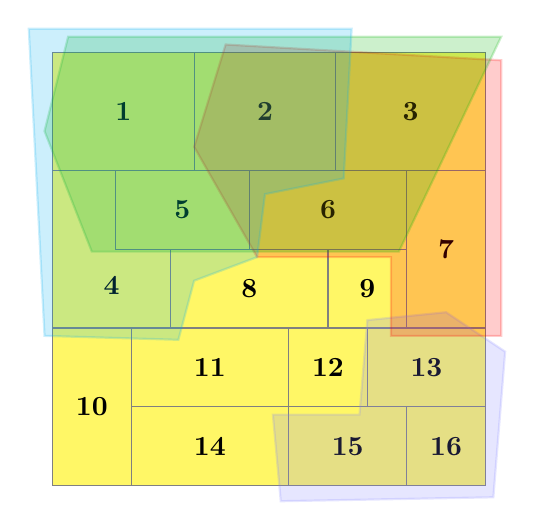
\begin{tikzpicture}[thin,draw=gray,font=\bf,fill opacity=0.6, text opacity=1]
\draw[fill=yellow] (0,0) rectangle (1,2)node[midway]{10};
\draw[fill=yellow] (1,0) rectangle (3,1)node[midway]{14};
\draw[fill=yellow] (3,0) rectangle (4.5,1)node[midway]{15};
\draw[fill=yellow] (4.5,0) rectangle (5.5,1)node[midway]{16};
\draw[fill=yellow] (1,1) rectangle (3,2)node[midway]{11};
\draw[fill=yellow] (3,1) rectangle (4,2)node[midway]{12};
\draw[fill=yellow] (4,1) rectangle (5.5,2)node[midway]{13};
\draw[fill=yellow] (4.5,2) rectangle (5.5,4)node[midway]{7};
\draw[fill=yellow] (3.5,2) rectangle (4.5,3)node[midway]{9};
\draw[fill=yellow] (1.5,2) rectangle (3.5,3)node[midway]{8};
\draw[fill=yellow] (0,2) -- (1.5,2)node[midway,above=0.3cm]{4} -- (1.5,3) -- (0.8,3) -- (0.8,4) -| cycle;
\draw[fill=yellow] (0.8,3) rectangle (2.5,4)node[midway]{5};
\draw[fill=yellow] (2.5,3) rectangle (4.5,4)node[midway]{6};
\draw[fill=yellow] (0,4) rectangle (1.8,5.5)node[midway]{1};
\draw[fill=yellow] (1.8,4) rectangle (3.6,5.5)node[midway]{2};
\draw[fill=yellow] (3.6,4) rectangle (5.5,5.5) node[midway]{3};

% Regions
\draw[draw=blue!50,fill=blue!50, opacity=0.2,text opacity=1,thick] (2.9,-0.2) -- (5.6,-0.15) -- (5.75,1.7) -- (5,2.2) -- (4,2.1) -- (3.9,0.9) -- (2.8,0.9) -- cycle;%

\draw[draw=red,fill=red, opacity=0.2,text opacity=1,thick] (4.3,1.9) -- (5.7,1.9) -- (5.7,5.4) -- (2.2,5.6) -- (1.8,4.3) -- (2.6,2.9) -- (4.3,2.9) -- cycle;%,

\draw[draw=green!70!black,fill=green!70!black, opacity=0.2,text opacity=1,thick] (0.5,2.97) -- (4.4,2.97) -- (5.7,5.7) -- (0.2,5.7) -- (-0.1,4.5) -- cycle;

\draw[draw=cyan,fill=cyan, opacity=0.2,text opacity=1,thick] (-0.1,1.9) -- (1.6,1.85) -- (1.8,2.6) -- (2.6,2.9) -- (2.7,3.7) -- (3.7,3.9) -- (3.8,5.8) -- (-0.3,5.8) -- cycle;%

\end{tikzpicture}

\end{document}
